\begin{abstract}
We give explicit covering certificates for a first-return map of planar null
geodesics in an equal-mass Majumdar--Papapetrou spacetime. Both masses are one
and their coordinate separation is two. Five disjoint strips in three affine
section boxes satisfy entry and exit inequalities for the first positive
upward return to $z=0$. Two interval implementations, one using binary64
Taylor enclosures and the other CAPD with 160-bit MPFR intervals, validate
the same five coverings. They share the specified model, boxes and strips;
their agreement does not independently validate that shared input.
The resulting edge shift has
spectral radius $\ph=(1+\sqrt5)/2$. Hence a compact invariant set of the return
map has topological entropy at least $\log\ph$. The contribution is a
checkable, parameter-specific certificate and a bound per return; it is not a
claim of the first rigorous proof of chaos in a two-centre spacetime.
\end{abstract}

\section{Statement and scope}

Planar photon scattering in two-centre Majumdar--Papapetrou geometries has a
substantial symbolic and numerical literature. Contopoulos \cite{Contopoulos}
studied photon and particle orbits around two fixed extreme
Reissner--Nordstr\"om black holes, relating capture and escape to unstable
periodic orbits and Cantor-like initial-condition sets. Dettmann, Frankel
and Cornish \cite{DFC} used numerical Lyapunov exponents and fractal basin
boundaries to characterize chaotic motion in multi-black-hole spacetimes.
Cornish and Gibbons
\cite{CG} describe symbolic dynamics in a family of two-centre models, and
Shipley and Dolan \cite{SD} develop a detailed account of null scattering and
black-hole shadows. Our object is a specified first-return map, with rational
section data and interval certificates for whole sets of initial conditions.

Qualitative positive entropy for the continuous-time optical geodesic flow
on a compact invariant set also follows from the compact-core case of
Bolotin and Kozlov's Theorem 2.1 \cite{BK}. Appendix~\ref{app:core} gives our
application to the optical metric: the specified compact domain has Euler
characteristic $-1$ and three strictly geodesically convex boundary
components. This general result does not specify the present strips or a
bound per return. Our method follows the established covering-relation
approach \cite{ZG}, including its computer-assisted applications to the
H\'enon, R\"ossler and Lorenz systems listed in its introduction; the covering method
itself is not new. Entropy values with different word lengths or time
parametrizations are not treated as the same quantity.

The finite data below specify the claim completely. Write $N_O,N_A,N_B$ for
the affine boxes in Section~\ref{sec:boxes}, and $K_{ij}\subset N_i$ for the
five strips in Table~\ref{tab:strips}.

\begin{theorem}\label{thm:main}
For the equal-mass system and section defined in Section~\ref{sec:model}, the
first-return map $P$, whose domain requires return before departure from
$\operatorname{int}\mathcal D$, is defined and continuous on each closed
$K_{ij}$. All return segments remain in the interior of
\[
 \mathcal D=\{r_+\geq 1/5,\ r_-\geq 1/5,\ x^2+z^2\leq64\}.
\]
With one exit coordinate and one entry coordinate, the following covering
relations hold:
\begin{equation}\label{eq:five}
 K_{OO}\cov N_O,\quad K_{OA}\cov N_A,\quad K_{AB}\cov N_B,
 \quad K_{BO}\cov N_O,\quad K_{BA}\cov N_A.
\end{equation}
Each $K_{ij}$ also covers every listed successor strip $K_{jk}\subset N_j$,
so every transition of the matrix in \eqref{eq:matrix} is realized by a
covering relation. There is a nonempty compact set
$\Lambda\subset K_{OO}\cup K_{OA}\cup K_{AB}\cup K_{BO}\cup K_{BA}$ with
$P(\Lambda)=\Lambda$ such that
\begin{equation}\label{eq:entropy}
 h_{\mathrm{top}}(P|_\Lambda)\geq
 \log\frac{1+\sqrt5}{2}\geq0.481211825059603.
\end{equation}
\end{theorem}

The theorem is computer-assisted: its finite inequalities are established by
the two interval implementations described in Section~\ref{sec:computations}.
The topological deduction is a prose proof using covering relations
\cite{ZG}; no Lean formalization is supplied. The statement concerns these
parameters and this return map. It does not assert hyperbolicity, conjugacy,
a description of the full shadow, or a lower bound for a time-one flow map.

\section{Model and first-return domain}\label{sec:model}

Use signed Cartesian coordinates $(x,y,z)$, with the two centres at
$(0,0,\pm1)$. On the invariant plane $y=p_y=0$, set
\begin{equation}\label{eq:potential}
 r_\pm=\sqrt{x^2+(z\mp1)^2},\qquad
 \mathcal U=1+\frac1{r_+}+\frac1{r_-}.
\end{equation}
The metric is
$ds^2=-\mathcal U^{-2}dt^2+\mathcal U^2(dx^2+dy^2+dz^2)$.
Fix $p_t=-1$ and the null constraint
\[
 H=\tfrac12\bigl[-\mathcal U^2+(p_x^2+p_z^2)/\mathcal U^2\bigr]=0.
\]
This fixes the affine-time scale. In the null reduction, put
$v=(v_x,v_z)=(p_x,p_z)/\mathcal U^2$ and $Q=(x,z)$. The equations used in both
certificates are
\begin{equation}\label{eq:ode}
 Q'=v,\qquad
 v'=\frac2{\mathcal U}\bigl(\nabla\mathcal U
             -v(\nabla\mathcal U\mathbin{\cdot}v)\bigr),\qquad
 \frac{dt}{d\lambda}=\mathcal U^2,
\end{equation}
where prime denotes differentiation with respect to $\lambda$.
These agree with the planar null Hamilton equations in \cite[Section II.1]{SD}.
The identity
\begin{equation}\label{eq:null}
 (|v|^2)'=\frac4{\mathcal U}(\nabla\mathcal U\mathbin{\cdot}v)(1-|v|^2)
\end{equation}
preserves $|v|=1$. Equation~\eqref{eq:ode}, regarded as a smooth extension off
this hypersurface, is also used to propagate outer interval sets.

Parameterize the upward section by
\begin{equation}\label{eq:section}
 \iota(q,w)=(q,0,w,\sqrt{1-w^2}),\qquad |w|<1.
\end{equation}
For a section point whose solution stays in $\operatorname{int}\mathcal D$
until its next upward crossing, let $\tau(q,w)>0$ be its first such crossing
time and define
\[
 P(q,w)=\pi\Phi_{\tau(q,w)}(\iota(q,w)),\qquad
 \pi(x,z,v_x,v_z)=(x,v_x).
\]
The initial zero at $\lambda=0$ is excluded. The domain of $P$ consists of
points for which this finite first return exists before departure from
$\operatorname{int}\mathcal D$. The certificates establish this property on
all five closed strips, including their boundaries. The artificial boundary
of $\mathcal D$ is a validation boundary, not an event horizon.

\section{Exact boxes and strips}\label{sec:boxes}

Let $c_i\in\R^2$, $e_i^u,e_i^s\in\R^2$ and $r_i^u,r_i^s>0$ be the data in
Tables~\ref{tab:centres}--\ref{tab:frames}. Every displayed finite decimal in
these two tables is an exact rational number. Define
\begin{equation}\label{eq:chart}
 T_i=[\,r_i^u e_i^u\ \ r_i^s e_i^s\,],\qquad
 \psi_i(u,s)=c_i+T_i(u,s)^{\mathsf T},\qquad
 N_i=\psi_i([-1,1]^2).
\end{equation}
The superscripts identify the exit and entry coordinates; no eigenvector or
hyperbolicity assertion is implicit in the notation.

\begin{table}[ht]
\centering\small
\begin{tabular}{@{}c rr rr@{}}\toprule
$i$ & $c_{i,q}$ & $c_{i,w}$ & $r_i^u$ & $r_i^s$\\\midrule
$O$ & $2.264907835107$ & $0$ & $0.00015$ & $0.0015$\\
$A$ & $2.251945728135$ & $-0.003640514957$ & $0.000005$ & $0.0015$\\
$B$ & $2.089732323743$ & $0.058272583543$ & $0.00015$ & $0.003$\\\bottomrule
\end{tabular}
\caption{Exact centres and radii in the section coordinates $(q,w)$.}
\label{tab:centres}
\end{table}

\begin{table}[ht]
\centering\small
\begin{tabular}{@{}c cc@{}}\toprule
$i$ & $e_i^u$ & $e_i^s$\\\midrule
$O$ & $(0.9521671202,\ 0.3055777729)$ & $(0.9521671202,\ -0.3055777729)$\\
$A$ & $(0.9516691518,\ 0.3071250974)$ & $(0.9514626094,\ -0.3077643628)$\\
$B$ & $(0.9424498218,\ 0.3343476236)$ & $(0.9453262599,\ -0.3261261449)$\\\bottomrule
\end{tabular}
\caption{Exact frame vectors. They are used as given, without normalization.}
\label{tab:frames}
\end{table}

For an edge $ij$ in Table~\ref{tab:strips}, write its listed interval as
$[a_{ij},b_{ij}]$ and set
\[
 K_{ij}=\psi_i([a_{ij},b_{ij}]\times[-1,1]).
\]
In its own h-set chart, the exit coordinate is rescaled from
$[a_{ij},b_{ij}]$ to $[-1,1]$; the entry coordinate is unchanged.
The frame determinants are nonzero. Exact rational geometry checks give
positive gaps between the $q$-projections of $N_O,N_A,N_B$:
\[
 \begin{aligned}
 \operatorname{gap}(N_O,N_A)&=\frac{9959078963811}{10^{15}},\\
 \operatorname{gap}(N_O,N_B)&=\frac{1706270893627}{10^{13}},\\
 \operatorname{gap}(N_A,N_B)&=\frac{157804105879171}{10^{15}}.
 \end{aligned}
\]
The two strips within $N_O$, and the two within $N_B$, have separated exit
intervals. Consequently all five $K_{ij}$ are pairwise disjoint.

\begin{table}[ht]
\centering
\begin{tabular}{@{}c cc@{}}\toprule
Strip & Exit interval in $N_i$ & Entry interval\\\midrule
$K_{OO}$ & $[-1/16,\ 1/16]$ & $[-1,1]$\\
$K_{OA}$ & $[-117/256,\ -85/256]$ & $[-1,1]$\\
$K_{AB}$ & $[-1/16,\ 1/16]$ & $[-1,1]$\\
$K_{BO}$ & $[151/512,\ 215/512]$ & $[-1,1]$\\
$K_{BA}$ & $[-1/16,\ 1/16]$ & $[-1,1]$\\\bottomrule
\end{tabular}
\caption{The five disjoint source strips.}
\label{tab:strips}
\end{table}

\section{Finite covering conditions}\label{sec:cover}

Let $(\mathsf U_j,\mathsf S_j)=\psi_j^{-1}\circ P$ be target coordinates.
For each source strip $K_{ij}$, the following sufficient conditions are
checked on the entire indicated sets:
\begin{align}
 -1&<\mathsf S_j(\psi_i(u,s))<1
 &&(a_{ij}\leq u\leq b_{ij},\ -1\leq s\leq1),\tag{C1}\label{eq:c1}\\
 \mathsf U_j(\psi_i(a_{ij},s))&<-1,\qquad
 \mathsf U_j(\psi_i(b_{ij},s))>1
 &&(-1\leq s\leq1).\tag{C2}\label{eq:c2}
\end{align}
No point sampling is substituted for these quantified conditions.

\begin{lemma}\label{lem:cover}
Conditions \eqref{eq:c1}--\eqref{eq:c2}, together with continuity of $P$, imply
$K_{ij}\cov N_j$. They also imply $K_{ij}\cov K_{jk}$ for every listed strip
$K_{jk}\subset N_j$.
\end{lemma}
\begin{proof}
In normalized source coordinates let $F=(F_u,F_s)$ be the target-coordinate
map. The homotopy
$((1-t)F_u+2tu,(1-t)F_s)$ has no intersection with the target entry boundary.
On the two source exit edges its first component stays, respectively, below
$-1$ and above $1$. At $t=1$ the exit map is $u\mapsto2u$, of degree one.
This is a covering relation in the sense of \cite{ZG}.

For a target strip with exit interval $[a,b]\subset(-1,1)$, replace the first
target coordinate by $(\mathsf U_j-(a+b)/2)/((b-a)/2)$. A value below $-1$
remains below the new left exit, and a value above $1$ remains above the new
right exit. The entry coordinate is unchanged. The same homotopy argument
therefore applies.
\end{proof}

\begin{figure}[ht]
\centering
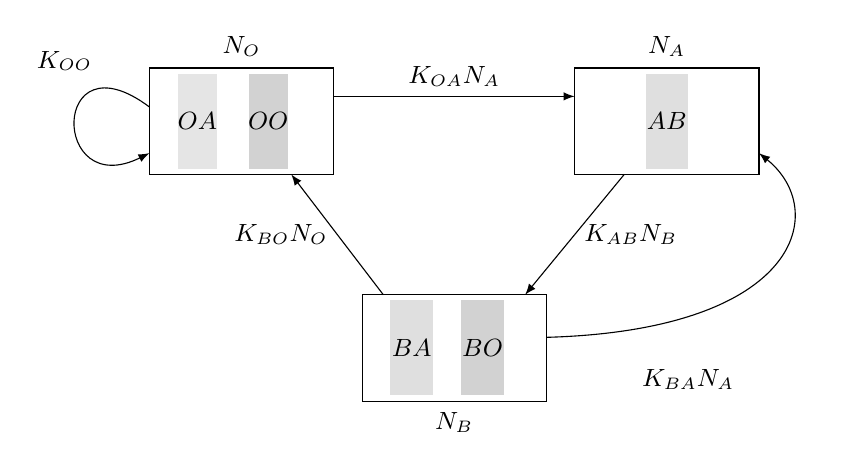
\begin{tikzpicture}[>=latex,scale=0.9,every node/.style={font=\small}]
\draw (-1.3,0) rectangle (1.3,1.5);
\node at (0,1.8) {$N_O$};
\fill[gray!20] (-.9,.08) rectangle (-.35,1.42);
\fill[gray!35] (.1,.08) rectangle (.65,1.42);
\node at (-.625,.75) {$OA$};\node at (.375,.75) {$OO$};
\draw (4.7,0) rectangle (7.3,1.5);\node at (6,1.8) {$N_A$};
\fill[gray!25] (5.7,.08) rectangle (6.3,1.42);\node at (6,.75) {$AB$};
\draw (1.7,-3.2) rectangle (4.3,-1.7);\node at (3,-3.5) {$N_B$};
\fill[gray!25] (2.1,-3.12) rectangle (2.7,-1.78);
\fill[gray!35] (3.1,-3.12) rectangle (3.7,-1.78);
\node at (2.4,-2.45) {$BA$};\node at (3.4,-2.45) {$BO$};
\draw[->] (1.3,1.1)--node[above] {$K_{OA}\cov N_A$}(4.7,1.1);
\draw[->] (-1.3,.95) .. controls (-2.7,2) and (-2.7,-.4) .. (-1.3,.3);
\node[align=center] at (-2.5,1.6) {$K_{OO}$};
\draw[->] (5.4,0)--node[right] {$K_{AB}\cov N_B$}(4,-1.7);
\draw[->] (2,-1.7)--node[left] {$K_{BO}\cov N_O$}(.7,0);
\draw[->] (4.3,-2.3) .. controls (7.9,-2.2) and (8.3,-.5) .. (7.3,.3);
\node at (6.3,-2.9) {$K_{BA}\cov N_A$};
\end{tikzpicture}
\caption{Schematic section boxes and their source strips; the geometry is not
to scale. An arrow denotes a covering from its labelled strip to the full
target box, hence to each successor strip. It does not assert a covering
from an entire parent box.}
\label{fig:scheme}
\end{figure}

\section{Two interval validations}\label{sec:computations}

Both computations use the exact input data above and the same definition of
first return. The first implements its own interval propagation and return
enclosure. The second uses CAPD's interval integrator and Poincar\'e map,
with a separately written model, initial-set construction, chart, tube audit
and acceptance predicates. Its recorded construction excluded the first
implementation's source and results (see \path{VERIFICATION-RECORD.md}),
but used the same frozen equations, boxes and strips. Errors in these shared inputs can affect both computations.
The two arithmetic choices, orders and subdivisions provide implementation
diversity, not independent selection of the geometric claim.

\subsection{Initial graph, existence and return isolation}

For each parameter cell, the full graph \eqref{eq:section} is enclosed. Its
nonlinear component uses the affine part of $g(w)=\sqrt{1-w^2}$ and a bound on
$g''(w)=-(1-w^2)^{-3/2}$. The common dependence on $(u,s)$ is retained in a
correlated set representation. Off-null points may be present in the outer
set, but \eqref{eq:null} ensures that the intended initial graph follows the
null dynamics.

Each implementation checks the integration tubes against the strict
inequalities $r_\pm>1/5$ and $x^2+z^2<64$. The initial upward departure is
excluded as a return, intervening crossings are distinguished by direction,
and the next upward crossing is isolated with strictly positive $v_z$.
In the binary64 computation, a sequence of sign states records departure,
the positive side, a strictly downward crossing, the negative side and the
strictly upward return window. On either side, a step is admitted only when
its tube avoids $z=0$ or its velocity sign excludes a new zero. Each crossing
window has a fixed nonzero sign of $v_z$ and opposite endpoint signs. This
proves that no earlier upward return was skipped. CAPD's oriented
Poincar\'e routine excludes the initial zero and locates the next
minus-to-plus crossing; an audit inside each integration step rejects every
section-intersecting tube for which $v_z$ can vanish. The recorded downward
crossing and positive return time exclude the initial departure.

For any initial point, departure and the isolated crossings are transverse;
the intervening closed orbit segments are separated from $z=0$. These
properties and the strict spatial margins persist under sufficiently small
changes of the initial point. Smooth dependence of the flow and the
implicit-function theorem at the final crossing therefore give continuity
of the first return on each closed strip. Only this continuity is used in
the covering argument.

\subsection{Binary64 implementation}

The first implementation uses Taylor order ten. Each basic arithmetic or
square-root result, evaluated in nearest rounding, is widened by one
representable number in each outward direction using \texttt{nextafter}.
The compiler options are \texttt{-O2 -ffp-contract=off -fno-fast-math};
the trust base includes correctly rounded binary64 operations and square
root. The base time step is $h=1/16$. Parameter rectangles are first split
to prescribed uniform width thresholds, then bisected further when an
enclosure or covering test remains unresolved. A strict Picard enclosure
proves existence on each time
step; Taylor remainder bounds enclose both the flow and its variational
matrix. Sets are represented as a centre, two correlated parameter columns,
and a moving four-dimensional error box. Approximate QR bases are permitted
because an interval enclosure of the inverse of the actual stored basis is
used in the inclusion update.

At the common time just before the return window, let the state be $X_0$
and its section coordinate be $z_0<0$. The positive lower bound for $v_z$
allows integration with respect to $z$. With
\[
 \mathcal L\supset\left(\frac{v_x}{v_z},\frac{v'_x}{v_z}\right)
 \quad\hbox{on the whole crossing tube},
\]
the return image satisfies
\[
 (x,v_x)_{\rm ret}\in(x,v_x)_0-\ell_0z_0+(\ell_0-\mathcal L)z_0
\]
for an arbitrary point vector $\ell_0$. Evaluating the first linear expression
in the correlated representation preserves useful cancellation. This
contains the images at the initial-condition-dependent hitting times, not
merely the state at a single common time.

The saved certificate has 768 accepted leaves across all fifteen conditions.
A separate exact-rational checker visits all 1521 nodes of the binary
partition trees and checks the recorded domain and crossing bounds and
strict target inequalities at every leaf. It audits saved bounds and does
not reintegrate the ODE.

\subsection{CAPD/MPFR implementation}

The second implementation uses CAPD 6.1 \cite{CAPD}, 160-bit MPFR intervals,
Taylor order 24 and the \texttt{MpC1Rect2Set} representation. Decimal inputs
are read with directed MPFR rounding. The interval Poincar\'e map uses the
upward orientation and an affine target-coordinate evaluation at an
interval-enclosed variable return time. An additional tube audit inside the
integration checks the
spatial boundary margins and rejects every section-intersecting tube whose
normal velocity contains zero. Positive return time, positive return
velocity and an audited downward crossing are also required.

All 2381 accepted records use the affine return enclosure in
\texttt{return\_check.cpp}, with condition labels C1, L and R. The
exploratory mean-value variant M1 contributes no accepted record.
Some accepted cells overlap or were retained from earlier subdivisions.
The saved-record checker is
\path{evidence/independent-capd/ab-extension/check_coverage.py}.
It validates rational cell indices in the unit parameter square, sweeps
their first-coordinate endpoints, merges overlapping second-coordinate
intervals in each slab, and sums exact rational areas. No clipping is
needed because the indices already constrain every cell to the square.
It checks the exit edges by interval unions. A finite union of closed
rectangles with full area covers the whole closed square: a nonempty
relative-open complement would have positive area. Thus the unions cover
each complete strip and both exit edges. This audit uses saved records,
without a new ODE integration. Unresolved parents are not accepted as evidence.
The numerical decision is made by native interval comparisons; printed
endpoints and derived margins are diagnostic values, checked separately.

\begin{table}[ht]
\centering\small
\begin{tabular}{@{}c cc c@{}}\toprule
Covering & Binary64 cells (C1; L; R) & CAPD cells (C1; L; R) & Result\\\midrule
$OO$ & $64;16;16$ & $128;16;16$ & C1, C2 pass\\
$OA$ & $64;16;16$ & $256;16;16$ & C1, C2 pass\\
$AB$ & $256;64;64$ & $1330;67;72$ & C1, C2 pass\\
$BO$ & $64;16;16$ & $272;16;16$ & C1, C2 pass\\
$BA$ & $64;16;16$ & $128;16;16$ & C1, C2 pass\\\bottomrule
\end{tabular}
\caption{Whole-set covering checks. Binary64 counts are partition leaves;
CAPD counts are distinct accepted parameter cells and need not form a
disjoint partition. The two counts are not a performance comparison.}
\label{tab:counts}
\end{table}

\begin{table}[ht]
\centering\small
\begin{tabular}{@{}c cc cc@{}}\toprule
 & \multicolumn{2}{c}{Binary64 conservative displayed bounds}
 & \multicolumn{2}{c}{CAPD diagnostic minima (approx.)}\\
Covering & C1 margin & C2 margin & C1 margin & C2 margin\\\midrule
$OO$ & $0.977$ & $11.422$ & $0.509499$ & $9.78842$\\
$OA$ & $0.402$ & $370.001$ & $0.161531$ & $320.784$\\
$AB$ & $0.500$ & $5.818$ & $0.000517844$ & $0.235386$\\
$BO$ & $0.339$ & $9.014$ & $0.000747296$ & $3.61244$\\
$BA$ & $0.920$ & $301.081$ & $0.317627$ & $135.569$\\\bottomrule
\end{tabular}
\caption{C1 margin means $1-\max|\mathsf S|$ for a cell enclosure. C2 margin
is the minimum of $-1-\sup\mathsf U$ on left cells and
$\inf\mathsf U-1$ on right cells. CAPD values come from \texttt{proof-summary.json}.
They are diagnostic values, not replacements for strict native interval
predicates.}
\label{tab:margins}
\end{table}

The CAPD source is
\path{evidence/independent-capd/ab-extension/proof-summary.json}.
The subdivision retains a cell as soon as its strict predicate passes,
without requiring a prescribed margin. Older overlapping cells can remain
in the final union. Its small minimum margins therefore depend on enclosure
width and subdivision history; they are neither robustness radii nor a
measure of disagreement between implementations. The two saved audits agree
on exact inputs and all fifteen covering conditions. No pointwise
intersection test of their return enclosures has been performed. The file
\path{evidence/independent-capd/review-audit.json} identifies every minimizing
task, original file, row and complete numerical output line.

For scale, the binary64 certificate encloses all return times in the
respective rational intervals
\[
\begin{array}{c|ccccc}
 ij&OO&OA&AB&BO&BA\\\hline
 \tau&[15.288,15.296]&[15.274,15.284]&[19.070,19.110]&
 [15.099,15.114]&[15.085,15.100].
\end{array}
\]
These are outward coarsenings of its recorded bounds in affine time
$\lambda$. For each strip, the aggregate CAPD return-time range is contained in the
corresponding displayed interval. This comparison concerns aggregate time
ranges, not pointwise intersection of the two return-image enclosures.
Agreement of coverings does not require equality or nesting of enclosures.

\section{From coverings to entropy}\label{sec:entropy}

Order the strips as $OO,OA,AB,BO,BA$. Lemma~\ref{lem:cover} gives the transition
matrix
\begin{equation}\label{eq:matrix}
 B=\begin{pmatrix}
 1&1&0&0&0\\
 0&0&1&0&0\\
 0&0&0&1&1\\
 1&1&0&0&0\\
 0&0&1&0&0
 \end{pmatrix}.
\end{equation}
It is the edge matrix of
$A=\left(\begin{smallmatrix}1&1&0\\0&0&1\\1&1&0\end{smallmatrix}\right)$.
The disjoint objects needed for symbolic coding are the five strips, rather
than three parent boxes with two incompatible whole-box assertions.

\begin{proof}[Proof of Theorem~\ref{thm:main}]
The interval certificates give \eqref{eq:c1}--\eqref{eq:c2}, the first-return
property and the strict domain and crossing margins. The preceding
continuity argument and Lemma~\ref{lem:cover} prove \eqref{eq:five} and every
transition in \eqref{eq:matrix}.

A closed admissible word for $B$ satisfies the hypotheses of the
closed-chain covering theorem \cite[Theorem 9]{ZG}: each strip is a compact
h-set with one exit and one entry coordinate, its affine chart extends to a
homeomorphism of $\R^2$, $P$ is continuous on each closed source strip, and
every forward covering has degree $+1$. No inverse-map hypothesis is used.
The theorem gives a point in the prescribed strip interiors fixed by the
corresponding iterate of $P$. Disjointness of the strips makes its itinerary
exactly the prescribed periodic word. Its least period need not equal the
length of a nonprimitive word. The directed graph of
$B$ is strongly connected, so every finite admissible word extends to a
periodic one. Let $\Lambda$ be the closure of the union of such periodic
orbits. It is compact and contained in the union of the five strips.
Continuity gives $P(\Lambda)\subset\Lambda$; taking convergent subsequences of
predecessors on the periodic orbits gives the reverse inclusion.

Because the strips are disjoint compact sets, recording the strip occupied
by each forward iterate defines a continuous itinerary map from $\Lambda$
to the full five-symbol one-sided space. Limits of the periodic itineraries
lie in its closed admissible subshift $\Sigma_B^+$, so the itinerary of every
point of $\Lambda$ is admissible. Periodic extensions of longer and longer
prefixes, followed by a compactness subsequence, realize every admissible
one-sided itinerary. This map to $\Sigma_B^+$ is onto
and intertwines $P$ and the shift. Therefore
$h_{\mathrm{top}}(P|_\Lambda)\geq h_{\mathrm{top}}(\sigma|_{\Sigma_B^+})
=\log\rho(B)$. Equivalently, distinct admissible words give orbit segments
separated by the positive distance between the strips, and their exponential
growth rate is $\rho(B)$.

All graph calculations can be performed over $\mathbb Q(\ph)$ with
$\ph^2=\ph+1$. The strictly positive vector
$\xi=(\ph,1,\ph,\ph,1)^{\mathsf T}$ satisfies $B\xi=\ph\xi$.
The induced weighted maximum norm of $B$ is $\ph$, which gives
$\rho(B)\leq\ph$, while the eigenvalue gives the opposite inequality.
The saved integer calculations also give
$\det(\zeta I-B)=\zeta^3(\zeta^2-\zeta-1)$.
An integer-square-root enclosure supplies rational lower and upper bounds
for $\sqrt5$. Substitution into the positive-term series
\[
 \log\ph=2\sum_{k=0}^{\infty}
       \frac{(\sqrt5-2)^{2k+1}}{2k+1}
\]
and an explicit tail bound, all evaluated by rational arithmetic, yield
\[
 \log\ph\in[0.481211825059603,0.481211825059604].
\]
\end{proof}

\section{Reproducibility and limits}

The accompanying certificate package contains the paper sources,
finite evidence and offline checking tools. Its file inventory is fixed by
\path{MANIFEST.sha256}; citation and archive status are recorded in its README.
The packet fixes the exact inputs, numerical
sources, accepted records and hashes. Its offline checkers audit all binary
partition leaves or exact unions of accepted CAPD cells, and can be run
without a new ODE integration. Reproducing the numerical enclosures requires
the specified compiler/arithmetic environment for the first implementation
or the pinned CAPD/MPFR build for the second. These are different levels of
reproduction; checking a saved inequality is not a reimplementation of the
underlying interval integrator.

English method descriptions and the expected versus generated checker
filenames are listed in \path{evidence/README.en.md}. The recorded software
environment and timing information are summarized in
Appendix~\ref{app:environment}.

The numerical trust base includes each interval implementation, elementary
arithmetic and functions, compiler and execution environment. Neither the
integrators nor the topological argument are formally verified here. The
proposed formalization level is L0: the current argument combines executable
interval certificates with an external covering theorem, and a Lean
statement alone would not certify that interface. The correspondence between the two computations is detailed in
\texttt{CORRESPONDENCE.md}.

According to its publicly accessible abstract, Pantig \cite{Pantig} develops
a conditional symbolic framework for multi-black-hole photon scattering.
Our claim is the five explicit coverings and the stated bound per return.
A full-text comparison remains pending, so no exhaustive priority assessment
is made against that work.

\paragraph{Use of AI.}
AI tools, including Codex and Claude, were used in implementation, checking
records, literature triage and drafting. They are tools, not authors.
Submission remains subject to the named author's review and responsibility;
this draft has not undergone human peer review.

\appendix
\section{A compact optical core}\label{app:core}

Here is the application of \cite[Theorem 2.1]{BK} used for context in the
introduction. On $M=\R^2\setminus\{(0,1),(0,-1)\}$ take the smooth optical
metric $g_{\rm opt}=\mathcal U^4(dx^2+dz^2)$ as the base metric, with
potential $V=0$ and energy $h=1/2$. The Jacobi metric is then $g_{\rm opt}$.
There are no potential singularities on $M$, so $\Delta=\varnothing$ and
$A(\Delta)=0$. The domain $\mathcal D$ is a disk of radius $R=8$ with the
two open disks of radius $\varepsilon=1/5$ removed; hence
$\chi(\mathcal D)=-1$ and $0>2\chi(\mathcal D)$.

For the inward Euclidean unit normal $n$ and its signed Euclidean curvature
$k_e$, the optical geodesic curvature is
\[
 k_g=\mathcal U^{-2}(k_e-2\partial_n\log\mathcal U).
\]
On the outer circle, $k_e=1/R$ and $n$ points towards its centre. Since
$r_\pm\geq R-1$, $\mathcal U\geq1$ and
$\partial_r\mathcal U\geq-2/(R-1)^2$,
\[
 \mathcal U+2R\partial_r\mathcal U
 \geq1-\frac{4R}{(R-1)^2}=\frac{17}{49}>0.
\]
On either inner circle, $n$ points away from that hole's centre and
$k_e=-1/\varepsilon$. The other centre is at least $2-\varepsilon$ away,
and consequently
\[
 \mathcal U+2\varepsilon\partial_\varepsilon\mathcal U
 \leq 1-\frac1\varepsilon+\frac1{2-\varepsilon}
       +\frac{2\varepsilon}{(2-\varepsilon)^2}
 =-\frac{269}{81}<0.
\]
Thus $k_g>0$ on all three boundary components, in the inward-normal
convention of \cite{BK}. The energy and convexity hypotheses are satisfied.
The resulting compact positive-entropy set for the optical geodesic flow
is a qualitative consequence of that existing theorem. This argument is
our application of it, and supplies neither the five strip coverings nor
their numerical entropy bound per return.

\section{Recorded computation environment}\label{app:environment}

Both recorded environments were macOS 26.6.2 on arm64. The binary64 solver
used Apple clang 21.0.0 with the following options, recorded in
\path{evidence/hset-check/trials.json}:
\begin{quote}\small\ttfamily\raggedright
-std=c++17 -O2 -ffp-contract=off -fno-fast-math
\end{quote}
The CAPD build used Homebrew GCC 16.2.0, MPFR 4.2.2 and GMP 6.3.0.
CAPD 6.1 was fixed at source commit
\path{37057e5899bccaa6cd5701057b7e6ea5e232ef8b}; its source-archive hash and
complete compile/link argument arrays are in \texttt{environment-record.json}
under \path{evidence/independent-capd/}.
The numerical executable used the options
\begin{quote}\small\ttfamily\raggedright
-std=c++17 -O2 -frounding-math\\
-D\_\_USE\_NATIVE\_\_ -D\_\_HAVE\_MPFR\_\_
\end{quote}
and linked CAPD, MPFR and GMP. Although the library configuration selects
the NATIVE backend and enables multiprecision, this solver uses 160-bit
\texttt{MpInterval}, not native double intervals. The historical build
record specifies the architecture but not the CPU model.

CAPD uses Taylor order 24, a step-selection tolerance of $10^{-20}$ and a
maximum step of $0.2$. These select time steps; certified errors come from
interval Taylor enclosures rather than from the tolerance itself.
The recorded library build took $110.037$ seconds. The six saved runs
contributing accepted CAPD cells took, respectively,
$151.775$, $194.846$, $1977.723$, $198.666$, $121.747$ and $7251.217$
wall seconds, in the order listed in the environment record. These times
include unresolved adaptive ancestors and are neither summed CPU times nor
a benchmark against binary64. Exact task tuples, failed attempts and
individual timings are preserved with the packet; no new integration was
performed for this manuscript revision.

\begin{thebibliography}{9}
\bibitem{Contopoulos} G. Contopoulos,
\emph{Periodic orbits and chaos around two black holes},
Proceedings of the Royal Society of London A \textbf{431} (1990), 183--202.
\href{https://doi.org/10.1098/rspa.1990.0126}{doi:10.1098/rspa.1990.0126}.
\bibitem{DFC} C.~P. Dettmann, N.~E. Frankel and N.~J. Cornish,
\emph{Fractal basins and chaotic trajectories in multi-black-hole spacetimes},
Physical Review D \textbf{50} (1994), R618--R621.
\href{https://doi.org/10.1103/PhysRevD.50.R618}{doi:10.1103/PhysRevD.50.R618}.
\bibitem{CG} N.~J. Cornish and G.~W. Gibbons,
\emph{The tale of two centres}, Classical and Quantum Gravity
\textbf{14} (1997), 1865--1881.
\href{https://doi.org/10.1088/0264-9381/14/7/020}{doi:10.1088/0264-9381/14/7/020}.
\bibitem{SD} J.~O. Shipley and S.~R. Dolan,
\emph{Binary black hole shadows, chaotic scattering and the Cantor set},
Classical and Quantum Gravity \textbf{33} (2016), 175001.
\href{https://doi.org/10.1088/0264-9381/33/17/175001}{doi:10.1088/0264-9381/33/17/175001}.
\bibitem{BK} S. Bolotin and V. Kozlov,
\emph{Topological approach to the generalized $n$-center problem} (2017).
\href{https://arxiv.org/abs/1705.04671}{arXiv:1705.04671};
\href{https://doi.org/10.1070/RM9779}{doi:10.1070/RM9779}.
\bibitem{ZG} P. Zgliczy\'nski and M. Gidea,
\emph{Covering relations for multidimensional dynamical systems},
Journal of Differential Equations \textbf{202} (2004), 32--58.
\href{https://doi.org/10.1016/j.jde.2004.03.013}{doi:10.1016/j.jde.2004.03.013}.
\bibitem{CAPD} T. Kapela, M. Mrozek, D. Wilczak and P. Zgliczy\'nski,
\emph{CAPD::DynSys: a flexible C++ toolbox for rigorous numerical analysis
of dynamical systems}.
\href{https://arxiv.org/abs/2010.07097}{arXiv:2010.07097}.
\bibitem{Pantig} R.~C. Pantig,
\emph{Symbolic dynamics of multi-black-hole photon scattering},
Physica D \textbf{498} (2026), 135415.
\href{https://doi.org/10.1016/j.physd.2026.135415}{doi:10.1016/j.physd.2026.135415}.
\end{thebibliography}
